\documentclass{beamer}

\usepackage[utf8]{inputenc}

\beamertemplatenavigationsymbolsempty %removes navigation bar

\usepackage{tcolorbox}%for colored boxes

%\defbeamertemplate{footline}{centered page number}
%{%
%  \hspace*{\fill}%
%  \usebeamercolor[fg]{page number in head/foot}%
%  \usebeamerfont{page number in head/foot}%
%  Scott, \textbf{Osmond}, Otto%
%  \hspace*{\fill}\vskip2pt%
%}
%\setbeamertemplate{footline}[centered page number]

\defbeamertemplate{headline}{centered page number}
{%
  \vspace{0.1cm}
  \hspace*{\fill}%
  \usebeamercolor[fg]{page number in head/foot}%
  \usebeamerfont{page number in head/foot}%
  Scott, \textbf{Osmond}, Otto [\insertframenumber\,/\,\inserttotalframenumber] \hspace{0.1cm}%
%  \hspace*{\fill}
%  \vskip2pt%
}
\setbeamertemplate{headline}[centered page number]

\usepackage{tikz}

\title{Gametic selection, meiotic drive, sex ratio bias, and transitions b/w sex determination systems}
\author{Michael Scott$^1$, \textbf{Matthew Osmond}$^2$, Sarah Otto$^2$}
\institute{$^1$University College London \& $^2$University of British Columbia}
\date{Evolution 2017}
\titlegraphic{\vspace{3cm}} %lifts text up

\begin{document}

%%%%%%%%%%%%%%%%%%%%%%%%%%%%%%%%%%%%%%%%%%%%%%%%%
%\frame{\titlepage}
\begin{frame}[plain]
   \begin{tikzpicture}[overlay, remember picture]
      \node[anchor = south east] at (current page.south east) {
         \scalebox{-1}[1]{\includegraphics[width=0.5\textwidth]{IMAGES/Sally}}
      };
      \node[anchor = south west] at (current page.south west) {
         \includegraphics[width=0.35\textwidth]{IMAGES/MikePenguin}
      };
   \end{tikzpicture}
      \titlepage
\end{frame}
%%%%%%%%%%%%%%%%%%%%%%%%%%%%%%%%%%%%%%%%%%%%%%%%%

%%%%%%%%%%%%%%%%%%%%%%%%%%%%%%%%%%%%%%%%%%%%%%%%%
\begin{frame}
\frametitle{Sex determination systems are remarkably dynamic}
   \begin{tikzpicture}[overlay, remember picture]
\visible<1>{
      \node[anchor = center] at (current page.center) {
         \includegraphics[width=\linewidth, angle=0]{IMAGES/TreeOfSex}
      };
      \node[anchor = south east] at (current page.south east) {
         Bachtrog \textit{et al.} 2014
      };
      \node[anchor = center, yshift=-4cm] at (current page.center) {
         \includegraphics[width=\linewidth, angle=0]{IMAGES/BachtrogEtAl2014Title}
      };
}
\visible<2->{
         \node[anchor = center] at (current page.center) {
           \huge 2 main theories
	};
}
   \end{tikzpicture}
\end{frame}
%%%%%%%%%%%%%%%%%%%%%%%%%%%%%%%%%%%%%%%%%%%%%%%%%

%%%%%%%%%%%%%%%%%%%%%%%%%%%%%%%%%%%%%%%%%%%%%%%%%
\begin{frame}
\frametitle{Theory 1: Turnover caused by sex-ratio selection}
   \begin{tikzpicture}[overlay, remember picture]
\visible<2->{
      \node[anchor = west, text width = 0.5\linewidth, xshift=-0.5cm] at (current page.west) {
         \includegraphics[width=\linewidth, angle=0]{IMAGES/Hamilton1967Fig1}
      };
      \node[anchor = west, text width = 0.5\linewidth, yshift = -3.8cm, xshift=-0.25cm] at (current page.west) {
         \includegraphics[width=\linewidth, angle=0]{IMAGES/Hamilton1967Title}
      };
      \node[anchor = south west] at (current page.south west) {
         Hamilton 1967
      };
}
\visible<3->{
      \node[anchor = east, text width = 0.75\linewidth, yshift=-1.5cm] at (current page.east) {
         \includegraphics[width=\linewidth, angle=0]{IMAGES/KozielskaEtAl2010Fig1a}
      };
      \node[anchor = east, text width = 0.7\linewidth, yshift = 2cm] at (current page.east) {
         \includegraphics[width=\linewidth, angle=0]{IMAGES/KozielskaEtAl2010Title}
      };
      \node[anchor = south east, yshift=5.5cm] at (current page.south east) {
         Kozielska \textit{et al.} 2010
      };
}
   \end{tikzpicture}
\end{frame}
%%%%%%%%%%%%%%%%%%%%%%%%%%%%%%%%%%%%%%%%%%%%%%%%%

%%%%%%%%%%%%%%%%%%%%%%%%%%%%%%%%%%%%%%%%%%%%%%%%%
\begin{frame}
\frametitle{Theory 2: Turnover caused by sex-antagonistic selection}
   \begin{tikzpicture}[overlay, remember picture]
\visible<2->{
      \node[anchor = center] at (current page.center) {
         \includegraphics[width=0.9\linewidth, angle=0]{IMAGES/vanDoornKirkpatrick2010Fig2}
      };
      \node[anchor = center, yshift=-3.9cm, xshift=0cm] at (current page.center) {
         \includegraphics[width=0.9\linewidth, angle=0]{IMAGES/vanDoornKirkpatrick2010Title}
      };
      \node[anchor = south east] at (current page.south east) {
         van Doorn \& Kirkpatrick 2010
      };
}
   \end{tikzpicture}
\end{frame}
%%%%%%%%%%%%%%%%%%%%%%%%%%%%%%%%%%%%%%%%%%%%%%%%%

%%%%%%%%%%%%%%%%%%%%%%%%%%%%%%%%%%%%%%%%%%%%%%%%%
\begin{frame}
   \begin{tikzpicture}[overlay, remember picture]
         \node[anchor = center] at (current page.center) {
           \huge Sex-ratio \textbf{and} sex-antagonistic selection?
	};
   \end{tikzpicture}
\end{frame}
%%%%%%%%%%%%%%%%%%%%%%%%%%%%%%%%%%%%%%%%%%%%%%%%%

%%%%%%%%%%%%%%%%%%%%%%%%%%%%%%%%%%%%%%%%%%%%%%%%%
\begin{frame}
\frametitle{Haploid-diploid life-cycles}
   \begin{tikzpicture}[overlay, remember picture]
\visible<1->{
      \node[anchor = center, yshift=2cm] at (current page.center) {
	[pictures of haploids, or life cycles]
      };
}
\visible<2->{
      \node[anchor = center, text width = \linewidth] at (current page.center) {
	\textbf{Haploid selection: Gametic competition and meiotic drive}
      };
}
\visible<3->{
      \node[anchor = center, text width = \linewidth, yshift=-1cm] at (current page.center) {
	Biased transmission of gametes, typically sex-specific\\
	$\implies$ can impart both \underline{sex-ratio \textbf{and} sex-antagonistic selection}
      };
}
\visible<4->{
      \node[anchor = center, text width = 1.1\linewidth, yshift = -3cm] at (current page.center) {
         \begin{tcolorbox}[colback=blue!5!white,colframe=blue!75!black,title=Question]
	   How does haploid selection influence sex-determination turnover?
	\end{tcolorbox}	
      };
}
   \end{tikzpicture}
\end{frame}
%%%%%%%%%%%%%%%%%%%%%%%%%%%%%%%%%%%%%%%%%%%%%%%%%

%%%%%%%%%%%%%%%%%%%%%%%%%%%%%%%%%%%%%%%%%%%%%%%%%
\begin{frame}
\frametitle{Model}
   \begin{tikzpicture}[overlay, remember picture]
      \visible<1->{
         \node[anchor = east, text width = \linewidth, xshift=0.5cm] at (current page.east) {
	    \includegraphics[width=0.4\linewidth, angle=90]{IMAGES/BarfBag1}\\
	    \includegraphics[width=0.4\linewidth, angle=90]{IMAGES/BarfBag2}
%	    \includegraphics[width=0.4\linewidth, angle=0]{IMAGES/BarfBag1}
%	    \includegraphics[width=0.4\linewidth, angle=0]{IMAGES/BarfBag2}
	 };
      }  
%      \visible<2->{
%         \node[anchor = south east] at (current page.south east) {
%	    \includegraphics[width=0.3\linewidth]{IMAGES/LondonBar}
%	};
%      }
%infinite popn, random mating, non-overlapping generations
%3 loci (selected, ancestral, dominant novel), 2 alleles at each
%recursion equations, stability analyses, numerical simulations
      \visible<2->{
         \draw[thick] (2,-1.25) circle [radius=1, thick];
         \node[anchor = west, text width = 2.5cm, yshift = 0cm, xshift=-0.25cm] at (current page.west) {
	    \begin{enumerate} \item recursion equations \end{enumerate}
	};
%         \path[->,thick] (eqns) edge (7.3,2.75);	
      }
      \visible<3->{
         \draw[thick] (2.75,-3) circle [radius=0.75, thick];
         \node[anchor = west, text width = 3cm, yshift = -3cm, xshift=0cm] at (current page.west) {
	    \begin{enumerate} \setcounter{enumi}{1} \item resident equilibrium \end{enumerate}
	};
%         \path[->,thick] (eqns) edge (7.3,2.75);	
      }
      \visible<4->{
         \draw[thick] (3.5,-1) circle [radius=0.75, thick];
         \node[anchor = west, text width = 2.5cm, yshift = 0cm, xshift=4.5cm] at (current page.west) {
	    \begin{enumerate} \setcounter{enumi}{2} \item invasion analysis \end{enumerate}
	};
%         \path[->,thick] (8.5,-3) edge (3.5,-1);	
      }   
      \visible<5->{
         \draw[thick] (7.75,2.75) circle [radius=0.75, thick];
         \node[anchor = east, text width = 2.5cm, yshift = 2.5cm, xshift=-0.1cm] at (current page.east) {
	    \begin{enumerate} \setcounter{enumi}{3} \item Taylor series of leading eigenvalue \end{enumerate}
	};
%         \path[->,thick] (8.5,-3) edge (3.5,-1);	
      }   
   \end{tikzpicture}
\end{frame}	
%%%%%%%%%%%%%%%%%%%%%%%%%%%%%%%%%%%%%%%%%%%%%%%%%

%%%%%%%%%%%%%%%%%%%%%%%%%%%%%%%%%%%%%%%%%%%%%%%%%
\begin{frame}
   \begin{tikzpicture}[overlay, remember picture]
         \node[anchor = center] at (current page.center) {
           \huge 2 main results
	};
   \end{tikzpicture}
\end{frame}
%%%%%%%%%%%%%%%%%%%%%%%%%%%%%%%%%%%%%%%%%%%%%%%%%

%%%%%%%%%%%%%%%%%%%%%%%%%%%%%%%%%%%%%%%%%%%%%%%%%
\begin{frame}
\frametitle{Result 1: Turnover can \textcolor{red}{\textit{create}} sex-ratio bias} %ploidally antagonistic selection
   \begin{tikzpicture}[overlay, remember picture]
         \node[anchor = south, text width = \linewidth, yshift=-0.9cm] at (current page.south) {
%%	    \includegraphics[width=\linewidth, angle=0]{../Plots/Combination_Turnover}
	    \includegraphics[width=\linewidth, angle=0]{../Plots/Combination_TurnoverMeanFit_Tighter}
	 };
        \node[] at (3,3) {
           XY $\rightarrow$ ZW
        };
        \node[] at (9,3) {
           ZW $\rightarrow$ XY
        };
        \node[] at (6,3) {
           \textcolor{gray}{$r=0.5 \rightarrow R=0.05$}
        };        
%        \node[text width=4cm] at (3.5,3) {
%           $\begin{aligned}
%           XY &\rightarrow ZW\\
%           r=0.5 &\rightarrow R=0.05
%           \end{aligned}$
%        };
%        \node[] at (8.5,3) {
%           $\begin{aligned}
%           ZW &\rightarrow XY\\
%           r=0.5 &\rightarrow R=0.05
%           \end{aligned}$
%        };
       \node[rotate = 90] at (-0.5,-0.75) {
          Drive in males opposes selection in diploids
        };
%       \node[rotate = 90] at (-0.5,-2.5) {
%           ZW $\rightarrow$ XY
%        };
   \end{tikzpicture}
\end{frame}
%%%%%%%%%%%%%%%%%%%%%%%%%%%%%%%%%%%%%%%%%%%%%%%%%

%%%%%%%%%%%%%%%%%%%%%%%%%%%%%%%%%%%%%%%%%%%%%%%%%
%\begin{frame}
%   \begin{tikzpicture}[overlay, remember picture]
%      \visible<1->{
%         \node[anchor = center, text width = \linewidth] at (current page.center) {
%	 \includegraphics[width=\linewidth, angle=0]{../Plots/Combination_MeanFit}
%	 };
%      } 
%   \end{tikzpicture}
%\end{frame}
%%%%%%%%%%%%%%%%%%%%%%%%%%%%%%%%%%%%%%%%%%%%%%%%%

%%%%%%%%%%%%%%%%%%%%%%%%%%%%%%%%%%%%%%%%%%%%%%%%%
\begin{frame}
\frametitle{Result 2: Turnover despite \textcolor{red}{\textit{looser}} linkage}
   \begin{tikzpicture}[overlay, remember picture]
         \node[anchor = south, text width = \linewidth] at (current page.south) {
	    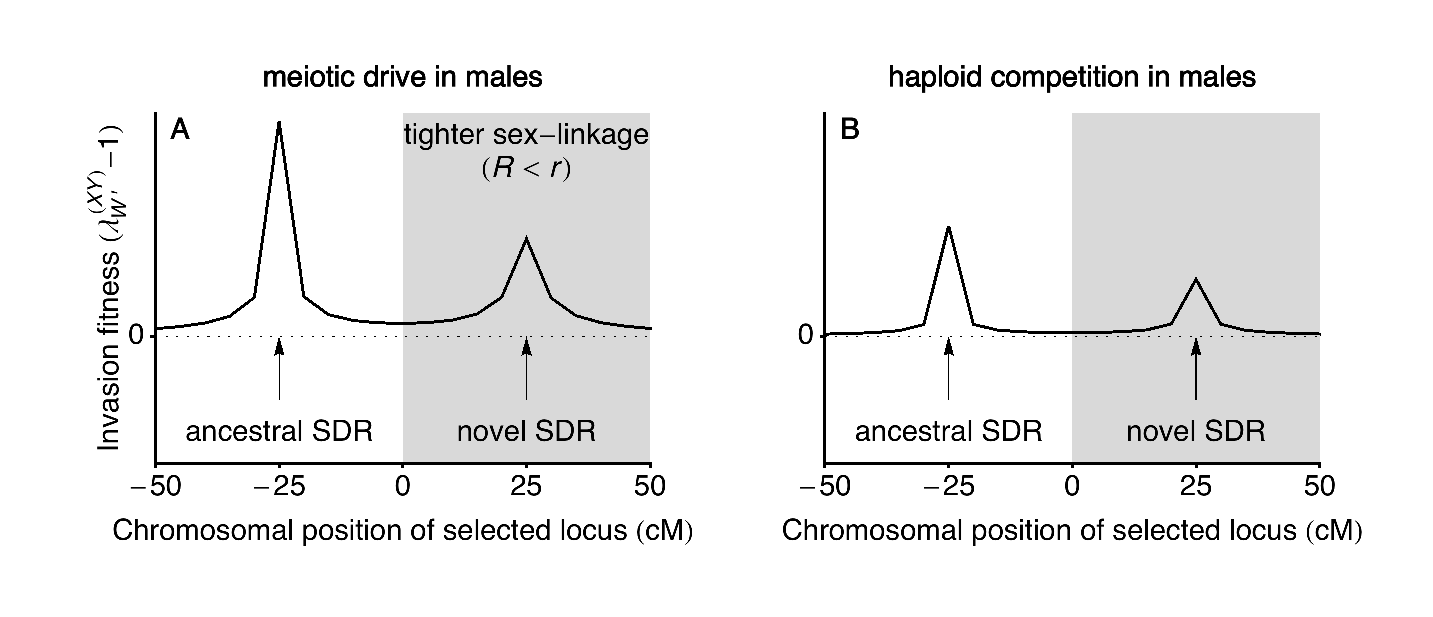
\includegraphics[width=\linewidth, angle=0]{../Plots/PositionPlot}
	 };
       \node[anchor=east] at (6,0) {
           sexually-antagonistic
        };
       \node[anchor=east] at (11,0) {
           drive opposes diploid sel$^n$
        };
       \node[anchor=east] at (6,-3.5) {
           ploidally-antagonsitic
        };
       \node[anchor=east] at (6,-1.25) {
           \textcolor{gray}{(stronger sel$^n$ in females)}
        };     
       \node[anchor=east] at (11,-3.5) {
           ploidally-antagonsitic
        };   
       \node[anchor=east] at (11,-1.25) {
            \textcolor{gray}{(stronger sel$^n$ in males)}
        };
       \node[anchor=center] at (7.3,3.4)  {
          \textcolor{gray}{ancestral SD}
        };
       \path[->,thick,gray] (7.3,3.2) edge (7.3,2.75);           
       \node[anchor=center] at (9.4,3.4) {
          \textcolor{gray}{novel SD}
        };                       
       \path[->,thick,gray] (9.4,3.2) edge (9.4,2.75);  
   \end{tikzpicture}
\end{frame}
%%%%%%%%%%%%%%%%%%%%%%%%%%%%%%%%%%%%%%%%%%%%%%%%%

%%%%%%%%%%%%%%%%%%%%%%%%%%%%%%%%%%%%%%%%%%%%%%%%%
\begin{frame}
\frametitle{Result 2b: Looser linkage evolves despite fitness \textcolor{red}{\textit{decline}}}
   \begin{tikzpicture}[overlay, remember picture]
         \node[anchor = south, text width = \linewidth, yshift=0cm] at (current page.south) {
	    \includegraphics[width=\linewidth, angle=0]{../Plots/Combination_TurnoverMeanFit_Looser}
	 };
        \node[] at (3,3) {
           XY $\rightarrow$ ZW
        };
        \node[] at (9,3) {
           ZW $\rightarrow$ XY
        };
        \node[] at (6,3) {
           \textcolor{gray}{$r=0.05 \rightarrow R=0.5$}
        };      
       \node[rotate = 90] at (-0.5,-0.75) {
          Drive in males opposes selection in diploids
        };          
   \end{tikzpicture}
\end{frame}
%%%%%%%%%%%%%%%%%%%%%%%%%%%%%%%%%%%%%%%%%%%%%%%%%

%%%%%%%%%%%%%%%%%%%%%%%%%%%%%%%%%%%%%%%%%%%%%%%%%
\begin{frame}
\frametitle{Bonus result! Turnover with very tight linkage}
   \begin{tikzpicture}[overlay, remember picture]
         \node[anchor = south, xshift=-1cm] at (current page.south) {
	    \includegraphics[width=0.75\linewidth, angle=0]{../Plots/regionplot_2b}
	 };
       \node[rotate = 90] at (-0.5,-0.75) {
          Overdominance in diploids, no haploid selection
        };
       \node[text width = 3cm] at (10,1) {
          \textcolor{red}{neo-W invades XY linked to X allele}
       };
       \node[text width = 3cm] at (10,-2) {
          \textcolor{blue}{neo-W invades XY linked to Y allele!}
       };                              
   \end{tikzpicture}
\end{frame}
%%%%%%%%%%%%%%%%%%%%%%%%%%%%%%%%%%%%%%%%%%%%%%%%%

%%%%%%%%%%%%%%%%%%%%%%%%%%%%%%%%%%%%%%%%%%%%%%%%%
\begin{frame}
\frametitle{Summary}
   \begin{tikzpicture}[overlay, remember picture]
      \visible<1->{
         \node[anchor = west, text width = 1.2\linewidth, yshift=2cm] at (current page.west) {
	    \begin{itemize}
	    \item Haploid selection creates new avenues for sex determination turnover
	    	\begin{enumerate}
	     	   \item Turnover can occur \textbf{regardless of sex-ratio bias}, and create it
	    	   \item Turnover can \textbf{decrease sex-linkage}, and mean diploid fitness
		   \end{enumerate}
	    \end{itemize}
       };                              
}
      \visible<2->{
         \node[anchor = west, text width = 1.2\linewidth, yshift=-2cm] at (current page.west) {
	    \begin{itemize}
	    \item Bonus result: Turnover possible with tight linkage, two mechanisms
	    	\begin{enumerate}
	     	   \item neo-W invades with X allele (female specialist)
	    	   \item neo-W \textbf{invades with Y allele} (from `perverse' overdominance equil.) 
		\end{enumerate}
	    \end{itemize}
	 };            
}
   \end{tikzpicture}
\end{frame}
%%%%%%%%%%%%%%%%%%%%%%%%%%%%%%%%%%%%%%%%%%%%%%%%%

%%%%%%%%%%%%%%%%%%%%%%%%%%%%%%%%%%%%%%%%%%%%%%%%%
\begin{frame}
\frametitle{Thank-you}
   \begin{tikzpicture}[overlay, remember picture]
         \node[anchor = west, text width = 0.4\linewidth] at (current page.west) {
   	    \centering
	    Michael Scott\\
	    \includegraphics[width=\textwidth]{IMAGES/MikePenguin}
	 };            
         \node[anchor = north east, text width = 0.4\linewidth, xshift=-4cm, yshift=-0.25cm] at (current page.north east) {
   	    \centering
            Otto lab\\
   	    \includegraphics[width=\textwidth]{IMAGES/OttoLab}
	 };     
         \node[anchor = east, text width = 0.4\linewidth, yshift=-0.75cm] at (current page.east) {
   	    \centering
            Sally Otto\\
   	    \includegraphics[width=\textwidth]{IMAGES/Sally}
	 };     
         \node[anchor = south west, yshift=0.7cm] at (current page.south west) {
   	    \includegraphics[width=0.5\textwidth]{IMAGES/BRC}
	 };     
         \node[anchor = south, xshift=1cm] at (current page.south) {
	    \includegraphics[width=0.15\textwidth]{IMAGES/UBC}
	 };     
         \node[anchor = south east, yshift=0.5cm] at (current page.south east) {	    			   \includegraphics[width=0.3\textwidth]{IMAGES/NSERC}
	 };   	   
   \end{tikzpicture}
\end{frame}
%%%%%%%%%%%%%%%%%%%%%%%%%%%%%%%%%%%%%%%%%%%%%%%%%

\end{document}